% \documentclass[Japanese]{dicomopapers}
\documentclass[Japanese,noauthor]{dicomopapers}

\usepackage[dvipdfmx]{graphicx}
\usepackage{latexsym}
\usepackage{amsmath}
\usepackage{url}

\def\Underline{\setbox0\hbox\bgroup\let\\\endUnderline}
\def\endUnderline{\vphantom{y}\egroup\smash{\underline{\box0}}\\}
\def\|{\verb|}
\def\newblock{\hskip .11em plus .33em minus .07em}

\begin{document}

% 和文表題
\title{ディスプレイを用いて光電脈波センサに\\任意の脈波を計測させる手法の提案}
% 英文表題
% \etitle{DICOMO2021 Paper Format (optional)}

% 所属ラベルの定義
\affiliate{Rits}{立命館大学大学院情報理工学研究科}
\affiliate{JST}{科学技術振興機構さきがけ}

\author{藤井 敦寛}{ATSUHIRO FUJII}{Rits}[atsuhiro.fujii@iis.ise.ritsumei.ac.jp]
\author{村尾 和哉}{KAZUYA MURAO}{Rits,JST}[murao@cs.ritsumei.ac.jp]

\begin{abstract}
  ウェアラブルデバイスに関する研究は活発に行われており,様々な形状,装着部位のデバイスが提案されている.ウェアラブルデバイスは自身の生体情報を記録するために利用される場合が多く,取得されたデータから身体異常を検知する手法などが提案されている.生体情報の中でも脈波データは感情推定などに利用されている.脈波センサは緑色のLEDを皮膚に照射して,血管を通して反射した光の変化から脈波を計測する光電式容積脈波記録法(PPG)と呼ばれる方式のものが一般的であり,スマートウォッチをはじめとする市販のウェアラブルデバイスに導入されている.脈波センサは機構の特性上,データの取得に血流を必要とするが,義手やロボットアームなど人工的な身体にスマートウォッチを装着する場合,血流が存在しないため正しいデータが取得できない.そこで,ディスプレイを用いて光電脈波センサに任意の脈波データを計測させる手法を検討する.本手法が実現すれば,身体と義手の接合部などで計測された脈波を入力することで,その値を義手に装着したスマートウォッチに読み取らせることが可能となる.本稿では心拍数に注目し,目標とする任意の心拍数を入力することでディスプレイを制御し,ディスプレイ上に装着したスマートウォッチで目標とする心拍数が取得できるか調査した結果について述べる.ディスプレイ描画プログラムとスマートウォッチアプリケーションを実装し,2台のディスプレイを使用して評価実験を行った.その結果,目標心拍数とスマートウォッチで計測された心拍数の誤差がDisplay Aでは平均-1.8回,Display Bでは平均-1.6回であり,全体では-3回以内と高い精度で心拍数を再現できた.しかしながら,脈波データの再現性は高くなかった.今後は実環境での使用を想定しながら再現性を高めつつ,身体から得られた脈波データを入力することでウェアラブルデバイスに同様の脈波データを計測させることができるように改良を重ねていく.
\end{abstract}

% 表題などの出力
\maketitle

% 本文はここから始まる
\section{はじめに}
\label{introduction}
健康管理への意識の高まりから,自身の生体情報を記録するウェアラブルデバイスが広く普及している.記録する生体情報は活動量や呼吸数,体温などさまざまな情報があり,脈波データや心拍数もそのひとつである.脈波データや心拍数を取得するために用いられる脈波センサは,緑色のLEDを皮膚に照射して,血管を通して反射した光の変化から脈波を計測する.心拍のタイミングで血流量が増加し,血管を通して反射した光が暗くなる.そして次の心拍まで血流量が減少していくため,反射する光が明るくなる.脈波データはこの反射光の変化の数値データであり,心拍数はこの明暗の変化のタイミングから計測される.この方式を光電式容積脈波記録法(PPG)と呼ぶ.スマートウォッチをはじめとする市販のウェアラブルデバイスの多くは,この方式を利用した脈波センサを搭載している.脈波データは生体情報の中でも重要なデータの一つであり,光電式容積脈波データを用いて呼吸数を推定する手法をHavriushenkoら\cite{respiratory_rate_estimation}が提案しているなど,脈波データを使用した研究は盛んである.\par

しかしながら,義手やロボットアームなど人工的な身体には血流が存在しないため,スマートウォッチを生身の身体と同様に手首に装着して生体情報を計測することはできない.通話やメッセージ,時計などのスマートウォッチの機能や加速度センサやGPSなどのセンサは人工的な身体でも利用できるが,生体情報の計測はできない.このように,人工的な身体において生身の身体で利用できていたインタフェース,デザイン,プロトコルが利用できない問題がある.この問題を解決するには,現状では追加のセンサを計測可能な身体部位に装着して,何からの通信手段を用いてセンサデータを収集する必要がある.しかし,仮に収集したとしても,スマートウォッチが提供するアプリにデータを与えてサービスを利用することはハードルが高いため,スマートウォッチに搭載されているセンサに計測させたい.しかし,計測可能部位にスマートウォッチを装着すると,本来のスマートウォッチとしての機能(時計やディスプレイ表示,タッチ操作)が利用できなくなるため,スマートウォッチ本来の使用形態である手首に装着して脈拍などの生体情報を計測できるようにすることが望ましい.\par

本研究では,ディスプレイを用いて光電脈波センサに脈波データを計測させる手法を検討する.ディスプレイの表示を変化させることで任意の脈波データを脈波センサに読み取らせることができれば,義手やロボットアームなどの人工的な身体にスマートウォッチを装着する場合でも,身体と義手の接合部などで計測された脈波を入力することで,その値をスマートウォッチに読み取らせることができ,スマートウォッチが提供する機能を生身の身体と同様に利用できる.また,人工的な身体にディスプレイを搭載するのみでスマートウォッチには手を加えないため,市販のスマートウォッチをそのまま利用できる.このほか,遠隔地のロボットアバタに適用すれば,操作者の生体情報をアバタの身体でも計測できるようになる.本稿では特にスマートウォッチへ任意の心拍数を入力することができるかを確認し,提案手法の有効性を明らかにする.\par

以降,\ref{sec:related}節で関連研究を紹介し,\ref{sec:method}節で提案手法の詳細を説明する.\ref{sec:preliminary}節で提案手法の実現可能性を調査するために行った予備実験について述べる.\ref{sec:evaluation}節で提案手法の評価を行い,\ref{sec:future_work}節で今後の計画を述べ,最後に\ref{sec:conclude}節で本研究をまとめる.



\section{関連研究}
\label{sec:related}
本節ではウェアラブルデバイスのセンシング,スマートウォッチの利用,脈波データの利用に関する研究を紹介する.

\subsection{ウェアラブルデバイスのセンシング}
Hamら\cite{smart_wristband}はスマートグラス用の入力デバイスとして,リストバンド型のデバイスを提案している.このデバイスはタッチパネルと慣性計測ユニットを搭載しており,タッチや手首をひねるなどのモーションで操作ができる.手首にデバイスを装着することで使用できるため,ユーザは動きを制限されず,自由度が高い.また,ポインティングにはタッチパネルを使用することで,入力の安定性を向上させた.
Hernandezら\cite{bioglass}は頭部装着型のウェアラブルデバイスである,Google Glassに内蔵された加速度センサ,ジャイロセンサ,カメラから脈拍数と呼吸数を認識する手法を提案している.
Nishajithら\cite{smart_cap}は,視覚障害者の状況認識を支援するウェアラブルデバイスとして,スマートキャップの設計と実装を行った.デバイスはRaspberry Pi 3,Raspberry Pi NoIR Camera V2,イヤホン,電源から構成される.Raspberry Pi NoIR(No Infrared) Camera V2とはRaspberry Piの赤外線カメラモジュールである.この赤外線カメラで得られる画像から検出された対象物について,イヤホンを通して音声で説明する.
これらはいずれも身体部位に装着するウェアラブルデバイスに関する研究であり,様々な形状のデバイスを用いた研究が行われている.\par

さらに,デバイスの装着部位も多岐にわたる.
Vahdatpourら\cite{localization_vahdatpour}は25人の被験者に頭部,胸部,両上腕,両前腕,腰部,両大腿部,両脛部の計10箇所に加速度センサを装着してもらい,日常行動下の加速度データを収集した.収集したデータからSVM(Support Vector Machine)を用いて,平均89\%の精度で装着部位を推定した.
Sztylerら\cite{localization_sztyler}は15人の被験者の頭部,胸部,左上腕,左手首,腰部,ズボンの左ポケット,左足首の計7箇所に加速度センサを装着し,様々な身体活動における加速度データを収集した.収集したデータからRandom Forestを用いて装着部位を推定し,平均89\%の精度を達成した.
Kunzeら\cite{localization_kunze}は6人の被験者の右手首,右目付近の側頭部,ズボンの左ポケット,左胸のポケットの計4箇所に加速度センサを装着し,歩行動作におけるデータを収集した.収集したデータからC4.5分類木を用いて装着部位を推定した.
また,筆者ら\cite{localization_yoshida}はウェアラブルデバイスで取得可能な生体情報である心電と脈波を利用し,特定の行動を装着者に行わせることなくウェアラブルデバイスの装着部位を推定する手法を提案している.\par

このように,ウェアラブルデバイスは様々な形状のものが提案されており,装着部位も広範囲であることから,活発な研究が行われている.


\subsection{スマートウォッチの利用}
ウェアラブルデバイスの中でもスマートウォッチは早くから市販化されていることもあり,多くの研究が行われている.
Spinsanteら\cite{accuracy_in_low_intensity}は低強度の身体活動時にスマートウォッチから取得される心拍数に注目し,その精度を計測している.
Senら\cite{eating_recognition}はスマートウォッチの加速度センサおよび,ジャイロセンサから得られるデータを使用して,手,箸,スプーンのいずれを使用して食べたかなどの食事行動を記録する手法を提案している.スマートウォッチ内蔵のカメラで食品画像を撮影し,画像識別を行うことにより食事内容も記録する.
Johnstonら\cite{smartwatch_walk_authentication}はスマートウォッチは常に同じ場所,同じ方向で身に着けることに着目し,スマートウォッチの加速度センサやジャイロセンサから得られるデータを使用して歩行に基づく生体認証を行う手法を提案した.一般的にスマートフォンはズボンのポケットやハンドバッグに格納して所持することが多い.これらの場所に比べ,スマートウォッチを装着する手首では活動の情報が大きく現れる傾向にある.
Weissら\cite{smartwatch_activity_recognition}は食事行動などの手に基づく身体行動において,スマートウォッチがスマートフォンよりも効果的に行動を識別できることを示した.``飲む''という行動において,スマートウォッチでは93.3\%の精度で識別できるのに対して,スマートフォンでは77.3\%の精度しか得られなかった.
Iakovakisら\cite{oh_detection}はスマートウォッチを用いて,姿勢変化による血圧(BP)の低下を予測することを目的とする研究を行っている.起立性低血圧(OH)はめまいや失神を引き起こす可能性があるとされており,高齢者だけでなく若年層でも転倒のリスクがある.そこで,心拍変動データを取得することで起立性低血圧による転倒リスクを低減する数学的予測モデルを提案している.
Mauldinら\cite{smartfall}は市販のスマートウォッチから得られる加速度データを用いて転倒を検知するAndroidアプリケーション``SmartFall''を提案している.スマートウォッチはSmartFallを実行するスマートフォンとペアリングされており,SmartFallはデータのプライバシーを守りつつクラウドサーバと通信し,転倒の予測に必要な計算をリアルタイムに実行する.
Ciabattoniら\cite{smartwatch_stress_detection}は様々な認知タスク中の精神的ストレスをリアルタイムに検出する手法を提案している.市販のスマートウォッチで取得したガルヴァニック皮膚反応(GSR),RR間隔,体温(BT)を用いてストレスを分類する.\par

人工的な身体ではウェアラブルデバイスを装着しても生体情報を収集できないため,これらの応用を利用できない可能性がある.加速度センサやGPSなどのセンサを用いた手法は適用できるが,生体情報を利用する手法は適用できない.これに対して筆者らは人工的な身体であったとしてもウェアラブルデバイスの生体情報センサにデータを計測させることで,生身の身体と同様にこれらの応用を利用できるようにすることを試みる.


\subsection{脈波データの利用}
Havriushenkoら\cite{respiratory_rate_estimation}はニューラルネットワークを用いて光電式容積脈波データから呼吸数の推定を行う手法を提案している.呼吸数を測定する方法としては,鼻腔内に設置した熱センサーや伸縮性のある胸部ベルトなどを用いることが多い.しかしながら,これらの方法は睡眠の妨げとなる可能性がある.脈波データを使用する手法であれば,ウェアラブルデバイスへの実装が可能である.検証の結果,2.2呼吸/分以下の平均呼吸数推定誤差を達成した.
% 今井ら\cite{fatigue_detection}はスマートウォッチの心拍データを用いて疲労度を検出する手法を提案している.スマートウォッチで疲労を検出できると,建設現場などで効果的な安全管理が期待できる.
Hanら\cite{arrhythmia_detection}はスマートウォッチから取得された光電式容積脈波データから心房期外収縮(PAC)および,心室性期外収縮(PVC)を検出する手法を提案している.
Goshvarpourら\cite{emotion_recognition_poincare}は単純な動的信号処理技術と統合手法から感情の変化を分類する手法を提案している.35人の被験者から安静時および,特定の感情を刺激するような音楽を聴いている状態で心電図と指の脈拍を収集した.ポアンカレプロットを使用した後にSVMを用いて幸福,悲しみ,安らぎ,恐怖の4つの感情に分類した.
Kajiwaraら\cite{pulse_order_picking}は多くの物流企業で手動でのオーダーピッキングシステムを採用しており,感情やエンゲージメントが作業効率やヒューマンエラーに影響を与えることに注目し,ウェアラブルデバイスで取得した行動や脈波から,運動強度の高い作業中における感情やエンゲージメントを予測する手法を提案している.脈波,眼球運動,動作を深層ニューラルネットワークに入力することで,感情やエンゲージメントの推定を行う.検証実験の結果,誤り率0.12以下の精度で予測できることを明らかにした.
Leeら\cite{fast_emotion_recognition}はPPGによる感情認識の速度向上に関する研究を行っている.行動価(valence)と覚醒度(arousal)に基づいた2次元の感情モデルを採用し,1D CNN(1次元畳み込みニューラルネットワーク)を用いることで,1.1秒のPPGデータから感情認識を行う.1D CNNを二値分類(行動価,覚醒度が高いか低いか)としてDEAPデータセットを用いて実験したところ,行動価では75.3\%,覚醒度では76.2\%の認識精度を達成した.\par

脈波データは身体の異常検知や感情推定ができるなど,重要な生体情報の一つである.市販のウェアラブルデバイスの脈波センサの多くは光電式容積脈波記録法(PPG)を使用している.そのため,血流の存在しない人工的な身体にウェアラブルデバイスを装着する場合,脈波データは取得できない.筆者らは生体情報の中でも脈波データに注目し,人工的な身体でも生身の身体と同様の脈波データをウェアラブルデバイスに計測させる手法を提案する.



\section{提案手法}
\label{sec:method}
本節では提案手法の詳細を述べる.


\subsection{概要}
\label{subsec:overview}
提案手法は任意の心拍数を何らかのインタフェースから入力すると,ディスプレイ上に装着したスマートウォッチでその心拍数が取得されるというものである.処理の流れを\figref{fig:method}に示す.まず,コンピュータに表示されているコンソールから取得したい心拍数を入力する.入力すると,その心拍数に応じた速度でコンピュータに接続されたディスプレイの明暗が変化する.そして,ディスプレイ上に装着したスマートウォッチで入力された心拍数が取得される.\par

ディスプレイの明暗の変化の制御は以下のように行う.
\begin{enumerate}
  \renewcommand{\labelenumi}{(\arabic{enumi})}
  \item 1回の脈拍を入力できるディスプレイの明暗の変化のデータ$Colors$を用意する
  \item 目標とする心拍数になるような速度で描画を繰り返す
\end{enumerate}

ここで,(1)におけるディスプレイの明暗の変化のデータは,事前調査から
\begin{equation*}
  \begin{split}
    Colors = [255, 255, 255, 255, 255, 255, 255, 255, 255, 255,\\250, 240, 232, 227, 225, 225, 229, 236, 245, 255]
  \end{split}
\end{equation*}
が本稿の段階では最適であることがわかっている.様々な値で実験した結果である.これはグレースケールのデータである.グレースケールとはコンピュータでの色の表現方法の一種であり,黒から白までの色の濃淡を$0$ ~ $255$の256段階で表現する.ディスプレイの明暗の変化のデータ$Colors$は次の流れで生成できる.
\begin{enumerate}
  \renewcommand{\labelenumi}{\arabic{enumi}.}
  \item $0$ ~ $2\pi$の間で20個等差に値を取る
  \item それぞれの値について$\sin$を取得する
  \item ぞれぞれの値に1を加える($0$ ~ $2$の範囲)
  \item 1以上の値を1に置き換える($0$ ~ $1$の範囲)
  \item ぞれぞれの値を30倍したあと,225を加える($225$ ~ $255$の範囲)
\end{enumerate}
このデータをプロットしたものを\figref{fig:colors_wave}に示す.光電式容積脈波記録法(PPG)を用いた脈波センサは,緑色のLEDを皮膚に照射して,血管を通して反射した光の変化から脈波を計測する.脈拍が発生するタイミングで血流量が増加するため,血管でより光が吸収される.すなわち,反射する光は暗くなる.これを再現しているのが,\figref{fig:colors_wave}の値が低下している部分である.グレースケールは値が小さくなるほど黒に近づく.黒は白に比べて光を吸収する.ディスプレイが黒く描画されるほど,ディスプレイ上に装着したスマートウォッチから発せられ,ディスプレイを通して反射する光は暗くなると考えられる.なお,\ref{sec:preliminary}節の予備実験で採用していたRGBからグレースケールへと変更した理由としては,(a)本質的には光の吸収度合いを制御することに意味があるため,その表示色自体に意味を持たない.(b)さまざまなディスプレイに対応できるよう,汎用性を高めるため.が挙げられる.\par

(2)では1分間で$Colors$を目標とする心拍数の回数だけ繰り返し描画する.値ごとの描画間隔$T_{wait}$は以下のように求める.
\begin{equation}
  \label{eqn:wait}
  T_{wait} = 60 / (L_{Colors} * TargetHeartRate)
\end{equation}
ここで,$L_{Colors}$は$Colors$のデータ長(本稿では20)であり,$TargetHeartRate$は目標心拍数である.$T_{wait}$ごとに$Colors$の値を1つずつ描画していく.

\begin{figure}[!t]
  \begin{center}
    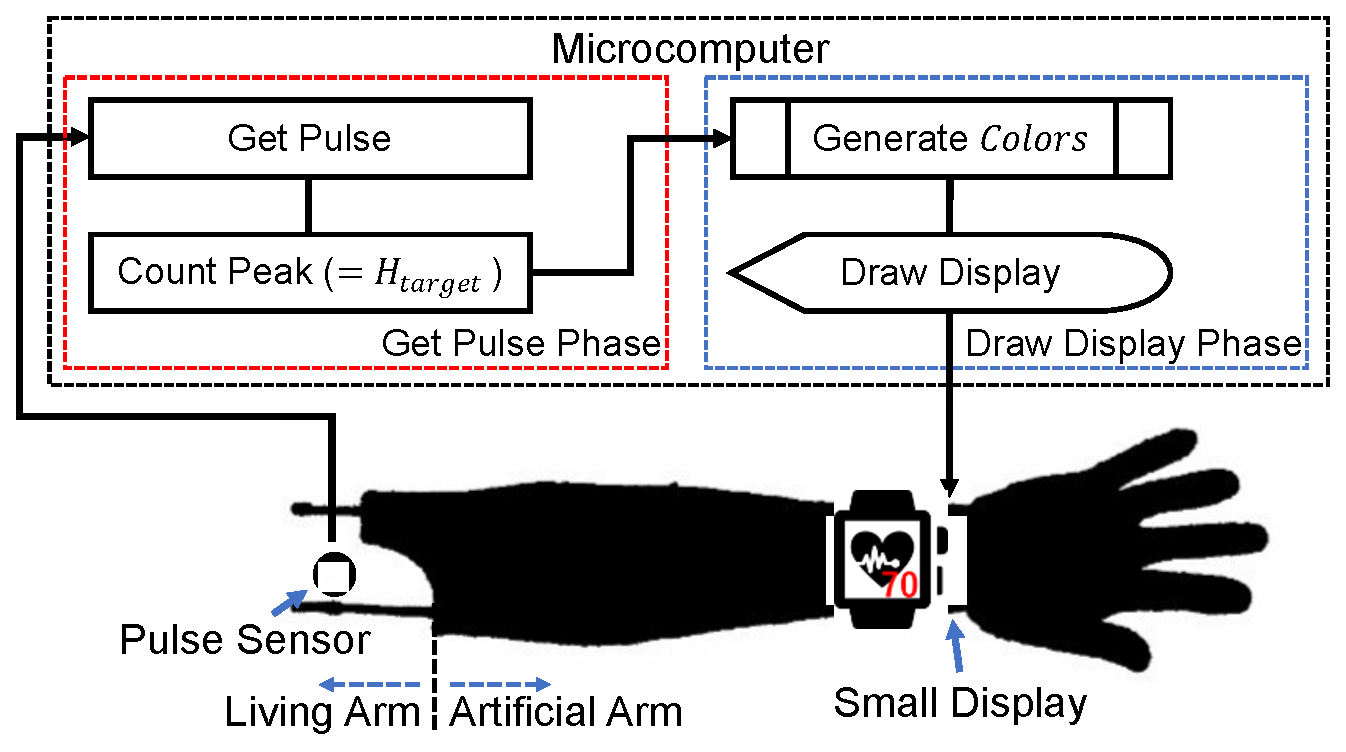
\includegraphics[width=1\linewidth]{figures/method.eps}
  \end{center}
  \caption{提案手法の処理の流れ}
  \label{fig:method}
\end{figure}

\begin{figure}[!t]
  \begin{center}
    \includegraphics[width=1\linewidth]{figures/colors_wave.eps}
  \end{center}
  \caption{1回の脈拍を入力できるディスプレイの明暗の変化のデータ}
  \label{fig:colors_wave}
\end{figure}


\subsection{ソフトウェア}
\label{subsec:software}
本節では提案手法を実装したソフトウェアの詳細を述べる.

\subsubsection{ディスプレイ描画プログラム}
\ref{subsec:overview}で述べたデータを作成し,ディスプレイに描画するプログラムをPythonとProcessingを用いて実装した.Processing\footnote{\url{https://processing.org}}とは視覚的な表現を得意とする,Javaをベースに開発されたプログラミング言語であり,電子アートやビジュアルデザインの作成などに使用される.実装したソフトウェアの処理の流れを\figref{fig:software}に示す.まず,Pythonで標準入力から目標とする心拍数を受け取る.データの作成部分ではNumpy\footnote{\url{https://numpy.org}}の\texttt{linspace}メソッドを用いて$0$ ~ $2\pi$の間で20個の値を取得し,\texttt{sin}メソッドでそれぞれの値についての$\sin$を取得し,さらに1加算する.ここで,1以上の値を全て1に置き換えることで$0$ ~ $1$の範囲の値とする.そして,それぞれの値を30倍して225加算することで,$225$ ~ $255$の値とする.ここで,式(\ref{eqn:wait})を用いて$T_{wait}$を計算しておく.作成した色データを1つずつPythonの\texttt{socket}ライブラリを使用してProcessingに送信し,描画の完了を待機する.Processing側ではデータを受信すると,そのグレースケールを\texttt{background}メソッドを使用して,ウィンドウの背景色として描画する.描画が完了したらPython側へ通知する.Python側で通知を取得すると現在時刻を取得し,あらかじめデータを送信する直前に取得しておいた$T_{now}$と比較を行い,$T_{wait}$が経過すると次の色データを送信する.この流れを繰り返し,$Colors$のデータを全て送信したら,再び$Colors$の1番目から同様にデータを取り出して処理を行う.

\begin{figure}[!t]
  \begin{center}
    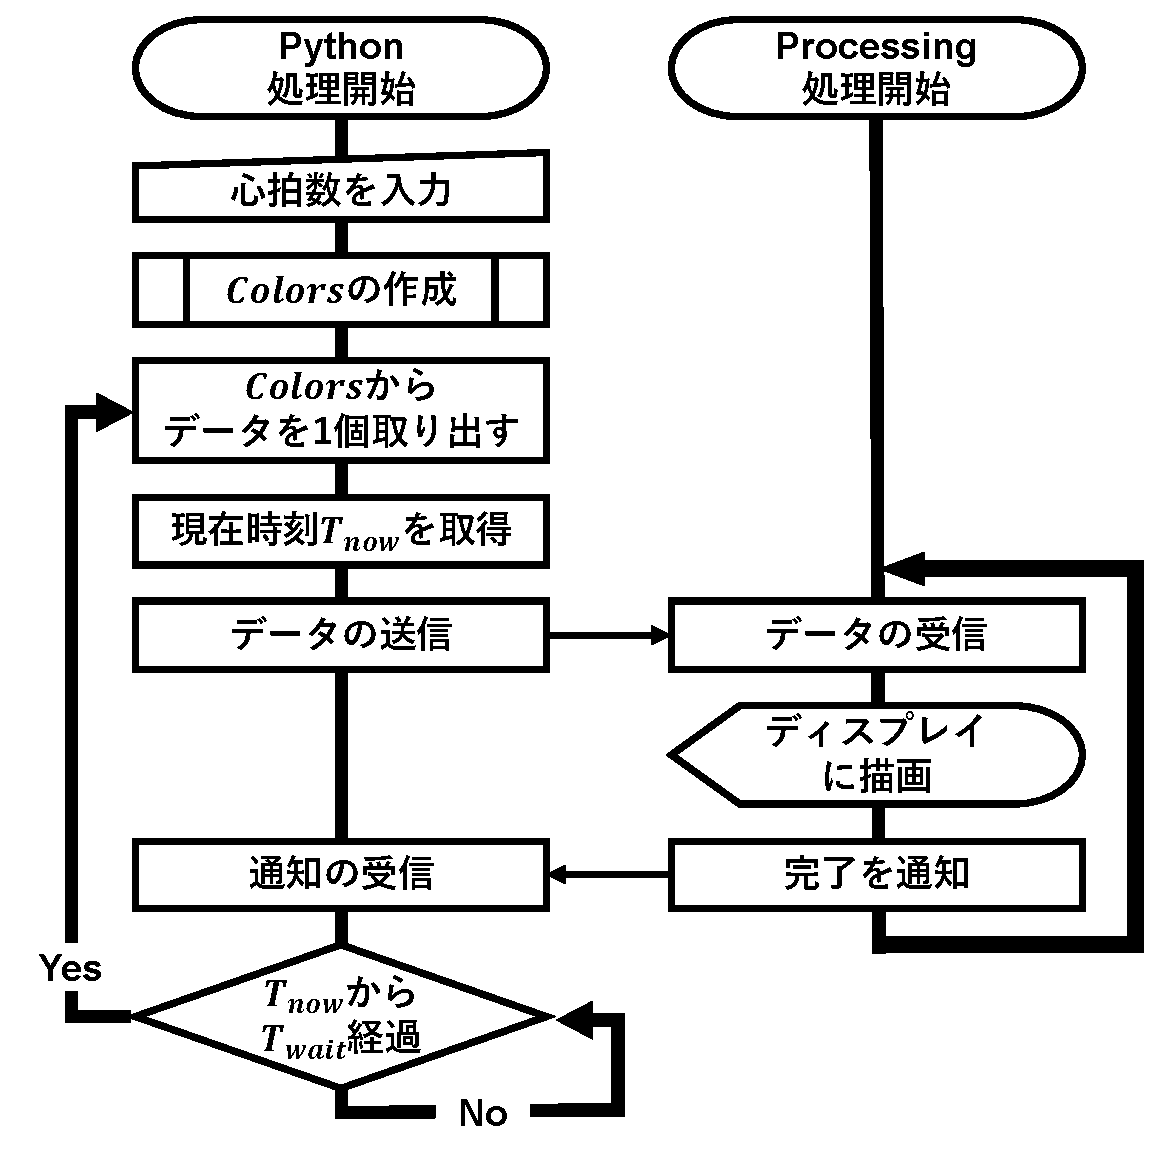
\includegraphics[width=1\linewidth]{figures/software.eps}
  \end{center}
  \caption{実装したプログラムの処理の流れ}
  \label{fig:software}
\end{figure}


\subsubsection{スマートウォッチアプリケーション}
心拍数を取得してスマートウォッチのディスプレイに表示し,データの記録を行うアプリケーションを実装した.今回は評価実験にGoogleのAndroidをベースにスマートウォッチ向けに設計されたOSであるWear OS by Google\footnote{\url{https://wearos.google.com}}を搭載したスマートウォッチを使用するため,Android Studioで実装した.実装したアプリケーションを\figref{fig:app}に示す.アプリケーションを起動すると,図中(1)の画面が表示される.センサ値の取得が自動的に開始され,値に変化があった場合,(2)のようにセンサ値が表示される.``Heart''は心拍数センサ,``Pulse''はPPGセンサの値を示す.データを記録する場合は``RECORD''ボタンを押下すると,(3)のように60秒間のキャリブレーションが開始される.このキャリブレーションは値の変動を安定させるために待機するものである.この間にスマートウォッチを固定しておく.60秒間のキャリブレーションが終了すると,(4)のように60秒間センサデータを取得し,変数に保存する.センサデータの取得時間が終了すると,変数に保存しておいたデータをcsv形式でスマートウォッチのストレージに保存し,(5)のように記録完了を示すメッセージが表示される.実装に使用したセンサの詳細について\tabref{tab:sensor_param}に示す.脈波データを取得するためのセンサ番号はデバイスにより異なる.ここでは評価実験に使用したTicWatch Pro WF12106(Mobvoi社製)でのセンサ番号を示す.サンプリングパラメータの``SENSOR\_DELAY\_UI''とは,ユーザインタフェースの実装に適したサンプリングレートである.\footnote{\url{https://developer.android.com/reference/android/hardware/SensorManager}}

\begin{figure}[!t]
  \begin{center}
    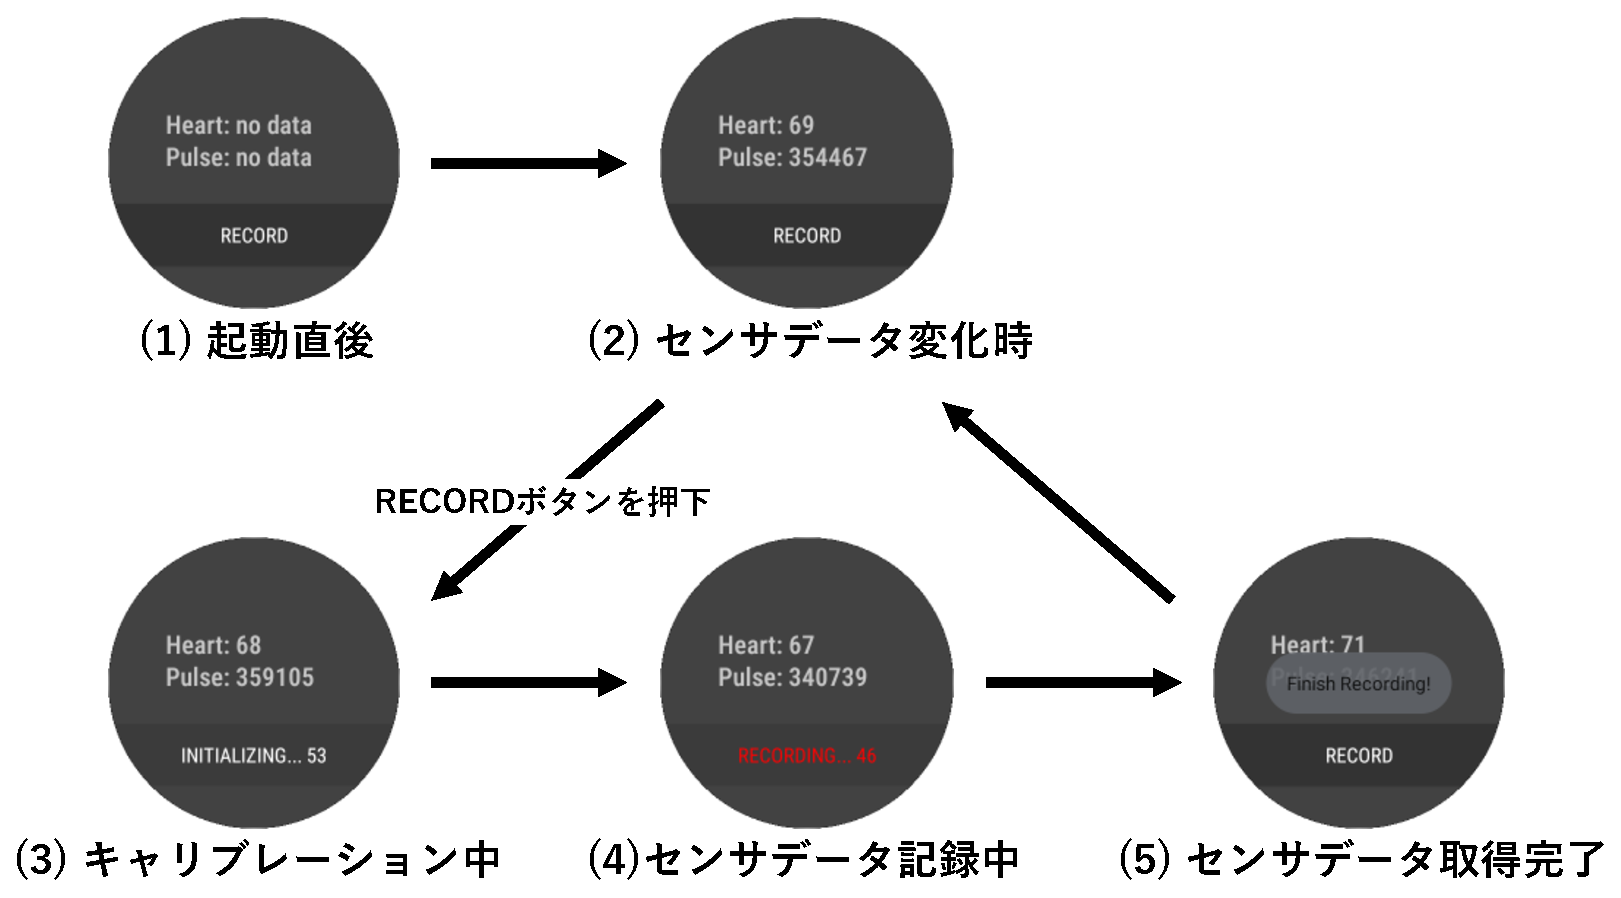
\includegraphics[width=1\linewidth]{figures/app.eps}
  \end{center}
  \caption{実装したアプリケーション}
  \label{fig:app}
\end{figure}

\begin{table}[!t]
  \centering
  \caption{実装に使用したセンサの詳細}
  \begin{tabular}{c|c|c} \hline\hline
    取得対象 & センサ番号 & サンプリングパラメータ \\ \hline
    心拍数 & 21 & SENSOR\_DELAY\_UI \\
    脈波データ & 65572 & SENSOR\_DELAY\_UI \\ \hline
  \end{tabular}
  \label{tab:sensor_param}
\end{table}



\section{予備実験}
\label{sec:preliminary}
本節では,提案手法の実現可能性を調査するため行った予備実験について説明する.ディスプレイ上に脈波センサを貼り付けた状態で,ディスプレイの色調を変化させたときの脈波センサの取得値を観察した.


\subsection{データ収集}
事前に実際の脈波データを筆者から収集した.\figref{fig:preliminary_sensors}の左図に示すように,左手人差し指に光電式容積脈波記録法の脈波センサ(pulsesensor.com製)を装着した.脈波センサはArduinoUNOを介してPCに接続しており,サンプリング周波数は約90Hzで10秒間データの収集を行った.

\subsection{実験方法}
データ収集で使用したPCとは異なるPC(Microsoft社製,SurfaceLaptop)のディスプレイの色調を変化させた.\figref{fig:preliminary_sensors}の右図に示すように,ディスプレイ上に脈波センサを乗せ,光が入らないように布で覆ったあと,ガムテープで固定した.事前に脈波データを収集したときと同じ条件でデータの取得を行った.ディスプレイの色調の変化にはJavaScriptを使用し,ブラウザの背景色を変化させることで制御した.事前に収集した脈波データを1サンプルずつ読み込み,その値に応じた3色で描画を繰り返す.全サンプルの処理が終了した場合,同じデータで再び処理を行う.
\par

描画する色は,次式により定義した.
\begin{equation}
	\label{eqn:low}
	value < \theta_{1} \quad (\theta_{1}=465)
\end{equation}

\begin{equation}
	\label{eqn:middle}
	\theta_{1} \leq value \leq \theta_{2} \quad (\theta_{1}=465, \theta_{2}=685)
\end{equation}

\begin{equation}
	\label{eqn:high}
	\theta_{2} < value \quad (\theta_{2}=685)
\end{equation}
式(\ref{eqn:low})を満たす場合はR:150, G:19, B:20,式(\ref{eqn:middle})を満たす場合はR:157, G:26, B:27,式(\ref{eqn:high})を満たす場合はR:156, G:25, B:26で表現される色を描画する.また,1サンプルを読み込み,色を描画するごとに10msの遅延を挟んだ.

\begin{figure}[!t]
	\begin{center}
		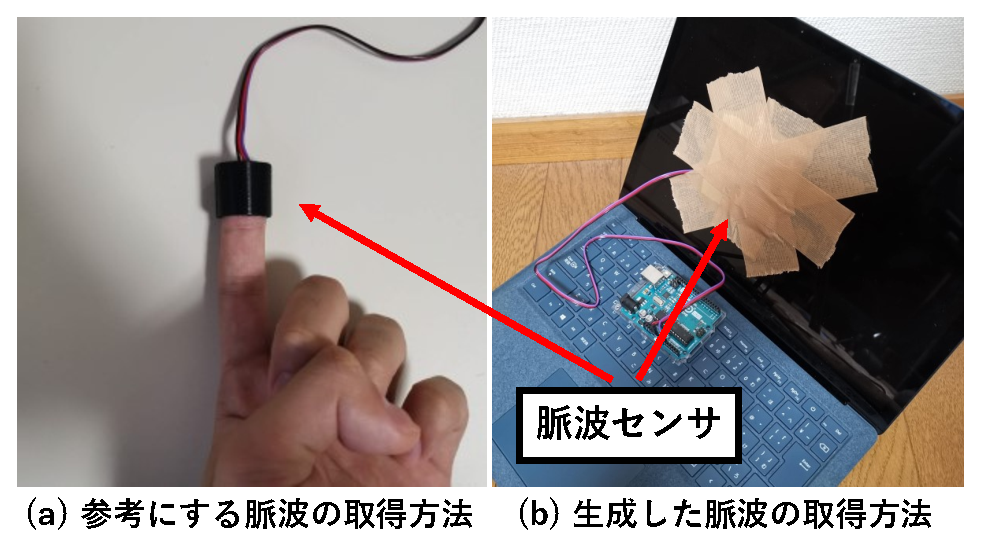
\includegraphics[width=1\linewidth]{figures/preliminary_sensors.eps}
	\end{center}
	\caption{予備実験での脈波データの取得方法}
	\label{fig:preliminary_sensors}
\end{figure}


\subsection{結果と考察}
取得された脈波データを,最初のピークから5秒間切り出した結果を\figref{fig:preliminary_pulse}に示す.結果から,ピークを生成できていることが確認できる.したがって,ディスプレイを使用するアプローチは有効だといえる.しかしながら,ピークの位置や値に違いが見られる.これは,ディスプレイ制御の開始時刻とセンサ値の取得の開始時刻を同期していなかったことや,サンプルの処理ごとの遅延を10msに固定していたことが影響したと考えられる.

\begin{figure}[!t]
	\begin{center}
		\includegraphics[width=1\linewidth]{figures/preliminary_pulse.eps}
	\end{center}
	\caption{脈波センサの取得値の変化}
	\label{fig:preliminary_pulse}
\end{figure}



\section{評価}
\label{sec:evaluation}
本節では,提案手法の効果を評価するために行った実験について説明する.特に心拍数に注目し,任意の目標となる心拍数を与えた際にスマートウォッチで取得される心拍数を観察した.


\subsection{データ収集}
\ref{subsec:software}節で実装したディスプレイ描画プログラムとスマートウォッチアプリケーションを使用してデータの収集を行う.スマートウォッチにはTicWatch Pro WF12106(Mobvoi社製)を使用し,ディスプレイはプログラムの実行に使用するノートPCであるLegion 7 15IMH05(Lenovo社製)の内蔵ディスプレイ(以下Display A)とマイクロコンピュータであるRaspberry Pi向けに設計された小型の3.5インチディスプレイ(OSOYOO社製)(以下Display B)を使用した.Display Bの接続にはHDMIを使用した.また,Display Bには購入時に画面を保護するためのフィルムが貼り付けてあったが,剥がした場合は正しくセンサ値が取得できなかったことから貼り付けたままの状態で実験を行った.心拍数データ取得のサンプリングレートは約1.03Hz,脈波データ取得のサンプリングレートは約20.69Hzである.データの取得は次の流れで行った.まず,実装したスマートウォッチアプリケーションを起動する.次にディスプレイ描画プログラムを実行し,適当な心拍数でディスプレイの描画を開始する.その状態でスマートウォッチをディスプレイに設置し,センサデータが更新されていることを確認する.このときの状態を\figref{fig:smartwatches}に示す.設置が完了したら,ディスプレイ描画プログラムの標準入力から目標心拍数を入力し,スマートウォッチアプリケーションの``RECORD''ボタンを押下する.60秒間キャリブレーションした後に,60秒間データ取得が行われる.目標心拍数を成人の平均心拍数である60回から100回\cite{heart_rate_average}まで5刻みで増加させながらデータを取得していき,100回に達すると再度60回から取得を繰り返す流れを3セット行う.以上の流れでディスプレイ2台でデータの取得を行った.

\begin{figure}[!t]
	\begin{center}
		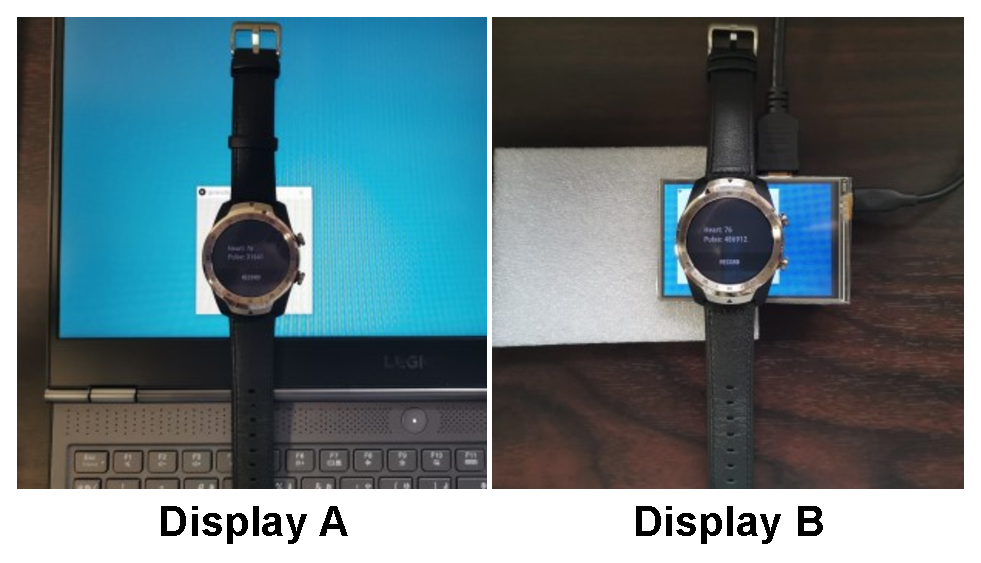
\includegraphics[width=1\linewidth]{figures/smartwatches.eps}
	\end{center}
	\caption{評価実験での心拍数の取得方法}
	\label{fig:smartwatches}
\end{figure}



\subsection{結果と考察}
データを取得した結果を\figref{fig:heartrate},\tabref{tab:heartrate}に示す.\figref{fig:heartrate}の横軸は目標心拍数で,縦軸は目標心拍数とスマートウォッチから取得された心拍数との誤差である.この誤差とは3セットでの平均値である.0は目標心拍数と一致していることを示し,マイナスは回数が不足していることを示す.\tabref{tab:heartrate}の``Average''はディスプレイごとの誤差の平均値である.\par

\tabref{tab:heartrate}の結果より,成人の平均心拍数である60回~100回において,目標心拍数よりおおよそ-3回以内の誤差でスマートウォッチに心拍数を入力できていることが確認できる.平均値ではあるが,目標心拍数を70回としたとき,Display Bを使用してスマートウォッチに心拍数を正しく入力できた.全体の平均としては目標心拍数よりDisplay Aでは1.8回少なく,Display Bでは1.6回少ないという結果となった.\par

また,\figref{fig:heartrate}の結果より,全体的に右肩下がりの傾向が見られる.目標心拍数が大きくなるほど,スマートウォッチで取得される心拍数はマイナス方向への誤差が大きくなっている.これは処理時間の同期の精度の低さや,ディスプレイのリフレッシュレートが関係していると考えられる.\figref{fig:method}のとおり,提案手法では$T_{wait}$ごとに色を更新していく必要があるが,PythonとProcessingでデータのやり取りなどもする必要があり処理時間により遅延が生じてしまい,本来ディスプレイに60秒間で描画すべき回数よりも描画回数が少なくなってしまっている可能性がある.この遅延時間は,処理回数が増加するのに伴って増加していくと考えられる.そのため,目標心拍数が大きくなるほど処理回数が増加し,それに伴いディスプレイへの描画の遅延が増加してしまい右肩下がりの傾向になったと考えられる.また,リフレッシュレートが低いと,正しく全ての色を$T_{wait}$ごとに描画できない可能性がある.リフレッシュレートについては,ディスプレイの性能に依存する.色データ$Colors$を調整することで,どのリフレッシュレートまで正しい心拍数を入力できるか,今後調査していく必要がある.\par

また実験中,ディスプレイ上にスマートウォッチを設置しても心拍数が0回となってしまい値が正しく取得できないことが何度も発生した.原因を調査するため,脈波データがどのような値であるかを観察した.ディスプレイ上で脈波を取得したときと同様のスマートウォッチアプリケーションで,筆者の左腕にスマートウォッチを装着して60秒間のデータを取得した.60秒間の平均心拍数は約68.3回だった.このデータを比較するために,最も近い心拍数である目標心拍数が70回のときのDisplay A,Bで取得した脈波データと共にプロットした結果を\figref{fig:pulse}に示す.なお,ディスプレイから得られた脈波データについては,それぞれ1セット目の取得時のデータである.横軸はデータの取得時刻であり,縦軸はセンサ値である.結果から,身体から得られた脈波と生成した脈波では大きく値が異なることが確認できる.そのため正しく心拍数が取得できなかったと考えられる.センサ値が小さいほどセンサと物質の距離が近い.腕部に装着したときはわずかながら隙間が存在する可能性があるが,ディスプレイ上に設置した場合は隙間が存在しない.そのため,腕部から得られた脈波よりもディスプレイから得られた脈波の方が値が小さくなったと考えられる.ディスプレイの種類によっても値に大きく差が存在することがわかる.これはディスプレイの材質,スマートウォッチの装着位置のズレなどにより反射率が変化したため,取得される値が変化したと考えられる.また,腕部より得られた脈波は脈拍による短周期の振れ以外にも,全体として緩やかに曲線状に波形が変化していることがわかる.これは身体部位に装着する場合はスマートウォッチが少なからず移動してしまい,装着位置がズレてしまうためであると考えられる.一方でディスプレイから得られた脈波は脈拍による短周期の振れは存在するものの,全体として直線状である.本実験ではディスプレイ上にスマートウォッチを置いた状態で値を取得した.置いた後は移動しないので,値はほぼ一定の間隔で変化すると考えられる.脈波データから感情推定を行う研究\cite{emotion_recognition_poincare}\cite{pulse_order_picking}\cite{fast_emotion_recognition}が存在するが,機械的な波形ではこれらの手法を適用しても正しい結果が得られない可能性がある.今後,より身体部位から得られた脈波への再現性を高めていく必要がある.

\begin{table}[!t]
  \centering
  \caption{スマートウォッチで取得された心拍数の誤差}
  \begin{tabular}{c|c|c} \hline\hline
    目標心拍数 & Display A & Display B \\ \hline
    60 & -1.0 & -1.0 \\
    65 & -1.3 & -1.3 \\
    70 & -1.0 & 0.0 \\
    75 & -2.0 & -1.7 \\
    80 & -2.0 & -2.0 \\
    85 & -2.0 & -2.3 \\
    90 & -2.0 & -2.0 \\
    95 & -2.0 & -1.7 \\
    100 & -2.7 & -2.3 \\ \hline
    Average & -1.8 & -1.6 \\ \hline
  \end{tabular}
  \label{tab:heartrate}
\end{table}

\begin{figure}[!t]
  \begin{center}
    \includegraphics[width=1\linewidth]{figures/heartrate_TicWatch.eps}
  \end{center}
  \caption{スマートウォッチで取得された心拍数の誤差}
  \label{fig:heartrate}
\end{figure}

\begin{figure}[!t]
  \begin{center}
    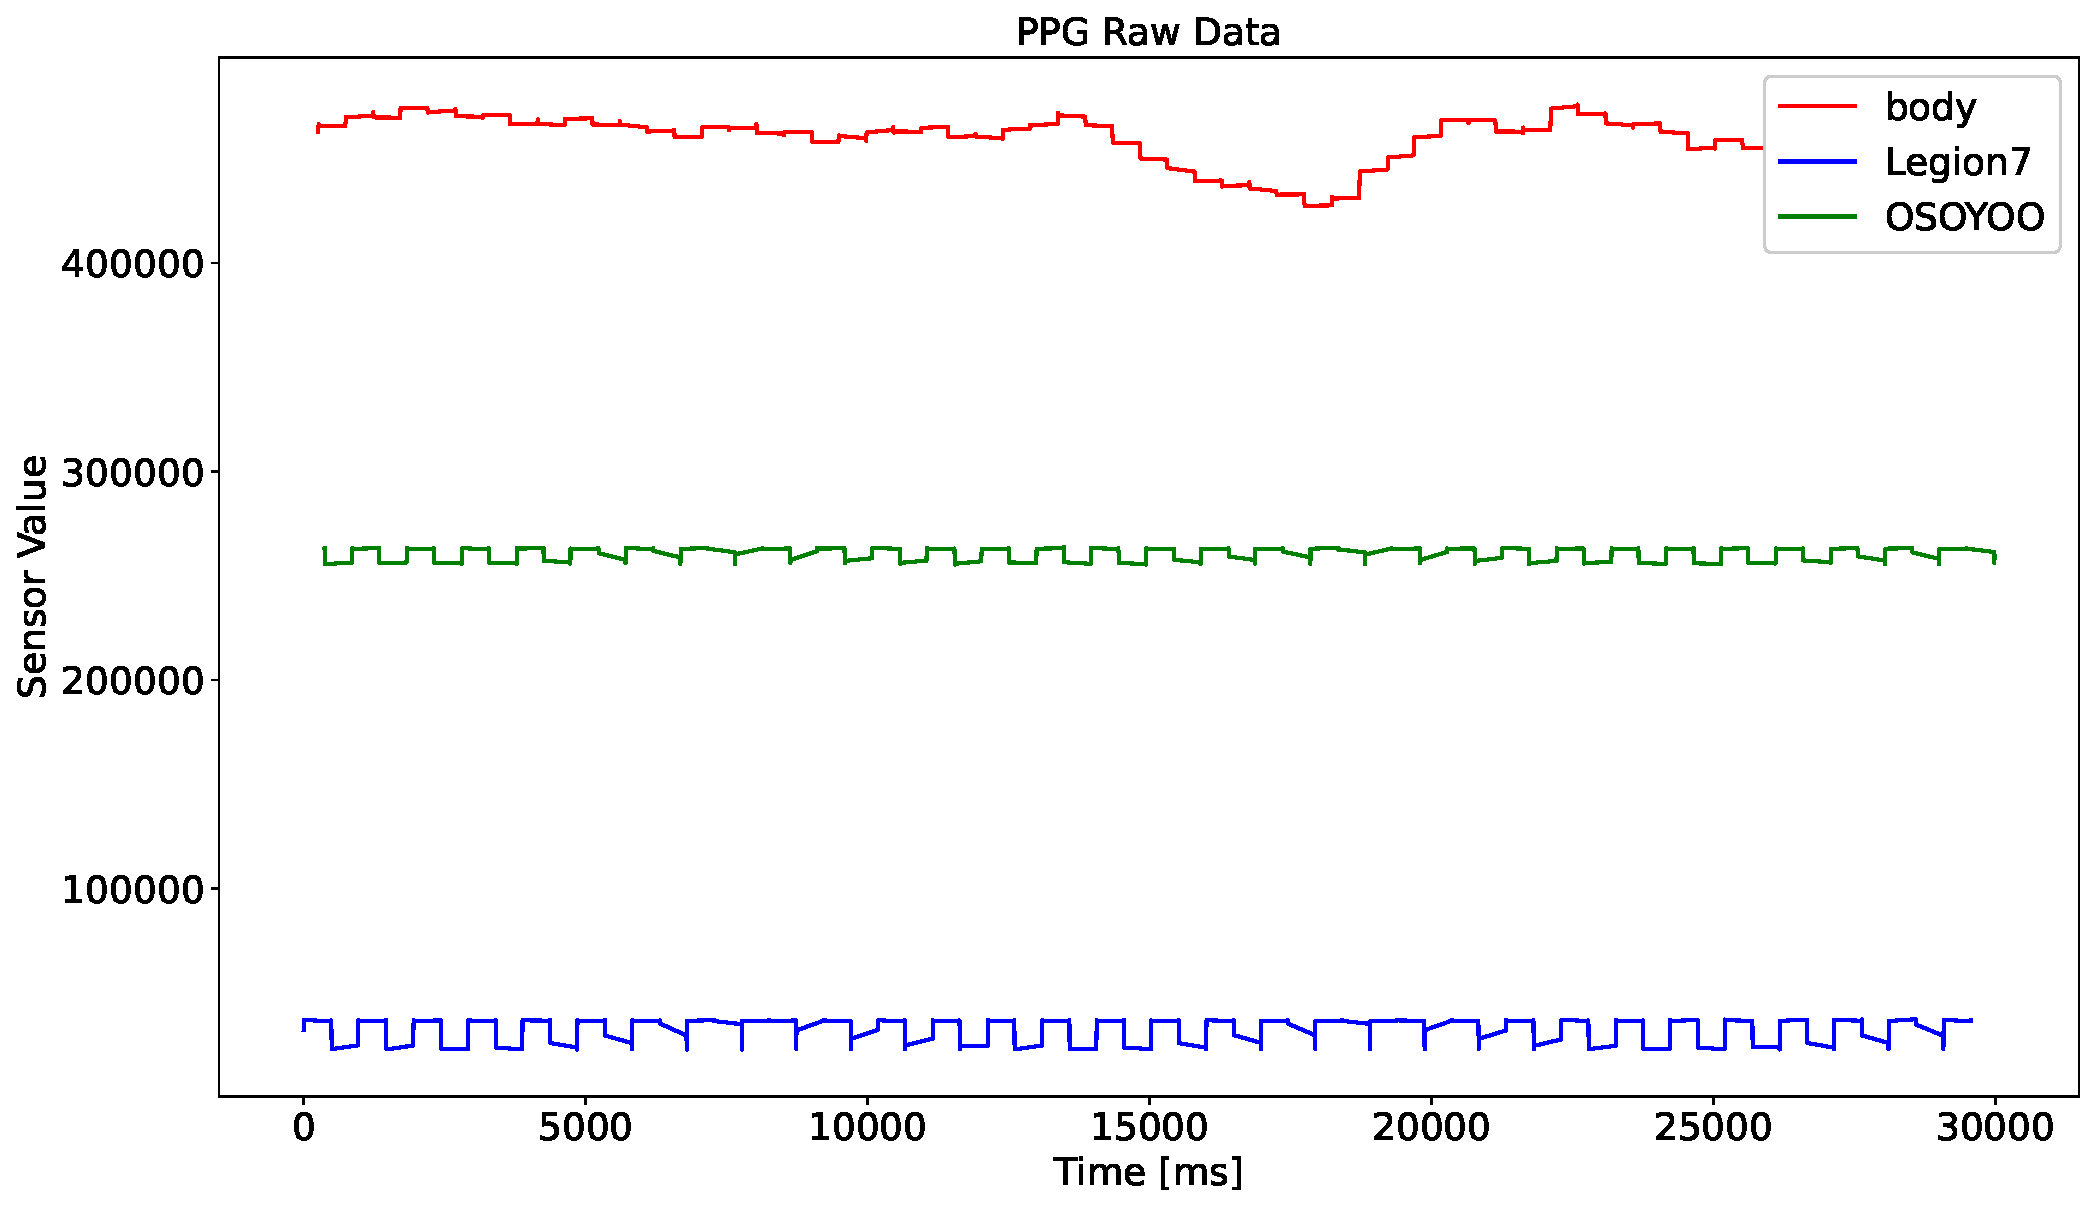
\includegraphics[width=1\linewidth]{figures/pulse_TicWatch.eps}
  \end{center}
  \caption{スマートウォッチで取得された脈波データ}
  \label{fig:pulse}
\end{figure}



\section{今後}
\label{sec:future_work}
評価実験ではディスプレイを用いてスマートウォッチに-3回以内の精度で,目標とする心拍数を計測させることができた.しかしながら,脈波データそのものの再現性の精度は高いとはいえない結果だった.また,ディスプレイに対する制約が存在するほか,装着位置によっても取得される値がシビアに変化してしまう.今後は実環境での使用を想定して脈波データの再現性を高めつつ,身体部位から得られた実際の脈波データを入力することで,ディスプレイ上に装着したウェアラブルデバイスに同一の脈波データを計測させる機構を実装する.この機構の想定を\figref{fig:future_work}に示す.実現するには,ディスプレイに描画する色を自動で決定し続ける必要がある.そのため,脈波データを入力することでディスプレイに描画する色を出力することができるような生成モデルを構築していく.また,身体部位に取り付けて使用することを想定し,デバイスの小型化を進めていくほか,複数のウェアラブルデバイスを使用して実験を行っていく.

\begin{figure}[!t]
  \begin{center}
    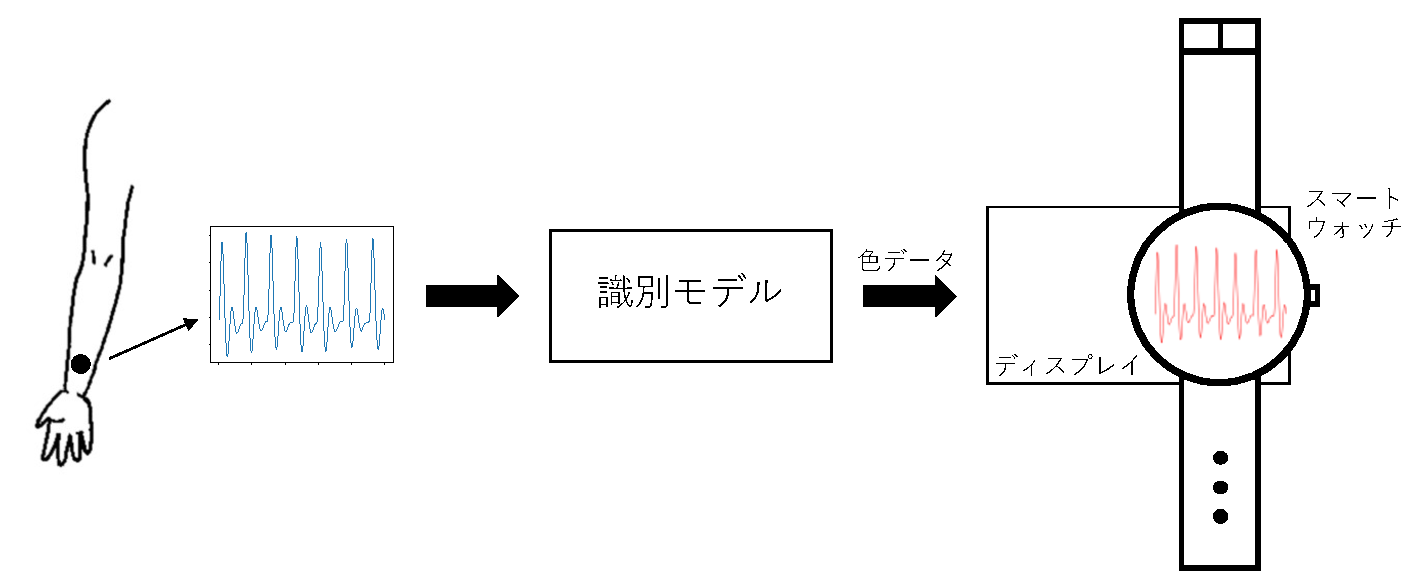
\includegraphics[width=1\linewidth]{figures/future_work.eps}
  \end{center}
  \caption{身体部位から得られた脈波データを入力し,再現する機構}
  \label{fig:future_work}
\end{figure}



\section{まとめ}
\label{sec:conclude}
本研究では,ディスプレイを用いて光電脈波センサに任意の脈波データを計測させる手法を提案した.評価実験を行う前に,提案手法の実現可能性を確認するために予備実験を行った.事前に筆者の実際の脈波データを収集しておき,そのデータから値に応じた色調をディスプレイに繰り返し描画しながら,ディスプレイ上に設置した脈波センサからデータを取得した.予備実験の結果,ディスプレイ上の脈波センサからピークの存在するデータが取得できた.したがって,脈波データを計測させるためにディスプレイを用いるアプローチは有効であるといえる.そこで,提案手法の効果を確認するために評価実験を行った.評価実験に必要なディスプレイ描画プログラムおよび,スマートウォッチアプリケーションを実装し,スマートウォッチとディスプレイ2台を使用して評価実験を行った.その結果,入力した目標心拍数と実際にスマートウォッチで取得された心拍数の誤差が,全体としては-3回以内だった.ディスプレイごとの平均では,Display Aでは-1.8回,Display Bでは-1.6回という結果であり,高い精度で心拍数が再現できた.\par

今後はディスプレイを用いることで,身体部位から取得された実際の脈波データと同様の脈波データをウェアラブルデバイスに計測させる機構を実装する.そのためには,自動でディスプレイの色調を決定していく必要があるため,適切な生成モデルを設計していく.また,身体部位への取り付けを想定し,デバイスの小型化を検討していく.



\begin{acknowledgment}
  本研究は,科学技術振興機構戦略的創造研究推進事業さきがけ(JPMJPR1937)の支援を受けたものである.ここに記して謝意を表す.
\end{acknowledgment}


\bibliography{references}
\bibliographystyle{junsrt}

\end{document}
